\chapter{Графовые модели}
\label{chap:gnns}

\begin{supportbox}{Об этой главе}
В этой главе мы рассматриваем данные с графовой структурой, т.е. узлы, соединенные набором (известных) отношений. Графы широко распространены в реальном мире, от белков до транспортных сетей, социальных сетей и рекомендательных систем. Мы представляем специализированные слои для работы с графами, в широком смысле разделяемые на слои передачи сообщений или архитектуры графовых трансформеров.
\end{supportbox}

\section{Обучение на графовых данных}
\subsection{Графы и признаки на графах}

До сих пор мы рассматривали данные, которые либо полностью неструктурированы (табличные данные, представленные в виде вектора), либо структурированы простыми способами, включая множества, последовательности и сетки, такие как изображения. Однако многие типы данных определяются более сложными зависимостями между их составляющими. Например, молекулы состоят из атомов, которые лишь разреженно соединены химическими связями. Сети многих видов (социальные сети, транспортные сети, энергетические сети) состоят из миллионов единиц (людей, продуктов, пользователей), которые взаимодействуют только через небольшой набор соединений, например, дороги, обратные связи или дружбу. Их более естественно определять на языке \textbf{теории графов}. Цель этой главы — представить дифференцируемые модели для работы с данными, определенными таким образом.

\begin{figure}[t]
    \centering
    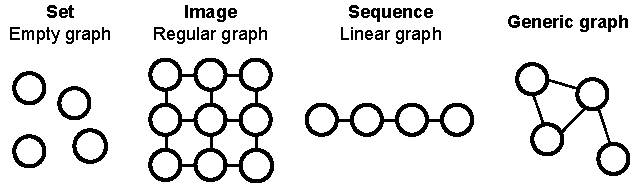
\includegraphics[width=0.8\textwidth]{images/graphs}
    \caption{Графы обобщают многие типы данных: множества можно рассматривать как пустые графы (или графы, имеющие только петли), изображения — как регулярные графы, а последовательности — как линейные графы. В этой главе мы рассмотрим более общие графовые структуры.}
    \label{fig:graphs}
\end{figure}

В своей простейшей форме граф можно описать парой множеств $\mathcal{G} = (\mathcal{V}, \mathcal{E})$, где $\mathcal{V} = \left\{1, \ldots, n\right\}$ — это множество \textbf{узлов} (\textbf{вершин}), а:
%
$$\mathcal{E} = \left\{(i,j) \mid \eqnmarkbox[drawred]{node}{i,j \in \mathcal{N}}\right\}$$
\annotate[yshift=-1em]{below,right}{node}{Два узла графа}

— это множество \textbf{ребер}, присутствующих в графе. В большинстве наборов данных количество узлов $n$ и количество ребер $m = \lvert \mathcal{E}\rvert$ могут варьироваться от графа к графу. 

Графы обобщают многие понятия, которые мы уже видели: например, графы, содержащие только \textbf{петли} вида $(i,i)$, представляют множества объектов, в то время как графы, содержащие все возможные ребра (\textbf{полносвязные графы}), связаны со слоями внимания, как мы покажем далее. Изображения можно представить в виде графа, связав каждый пиксель с узлом графа и соединив близкие пиксели на основе регулярной сеточной структуры - см. Рисунок \ref{fig:graphs}.\footnote{Существует много вариантов этой базовой схемы, включая гетерогенные графы (графы с разными типами узлов), ориентированные графы, знаковые графы и т.д. Большинство из них можно обработать с помощью вариаций техник, которые мы опишем далее.}

Соединения в графе можно эквивалентно представить матричным представлением, называемым \textbf{матрицей смежности}. Это двоичная квадратная матрица $\mathbf{A} \sim \text{Binary}(n,n)$, такая что:
%
$$
A_{ij} = \begin{cases} 1 & \text{ если } (i,j) \in \mathcal{E} \\ 0 & \text{ иначе} \end{cases}
$$
%
В этом формате множество представляется единичной матрицей $\mathbf{A} = \mathbf{I}$, полносвязный граф — матрицей из всех единиц, а изображение — матрицей Тёплица. Граф, в котором соединения всегда двунаправленные (т.е. $(i,j)$ и $(j,i)$ всегда присутствуют как пары среди ребер), называется \textbf{неориентированным}, и мы имеем $\mathbf{A}^\top = \mathbf{A}$. Для простоты мы будем иметь дело с неориентированными графами, но методы можно легко расширить на ориентированный случай. Мы отмечаем, что существуют и альтернативные матричные представления, например, матрица инцидентности $\mathbf{B} \sim \text{Binary}(n, \lvert \mathcal{E}\rvert)$ такова, что $B_{ij} = 1$, если узел $i$ участвует в ребре $j$, и мы имеем $\mathbf{B}\mathbf{1}^\top = 2$, потому что каждое ребро соединяет ровно два узла. См. Рисунок \ref{fig:adjacency_matrix} для примера.

\begin{figure}[t]
    \centering
    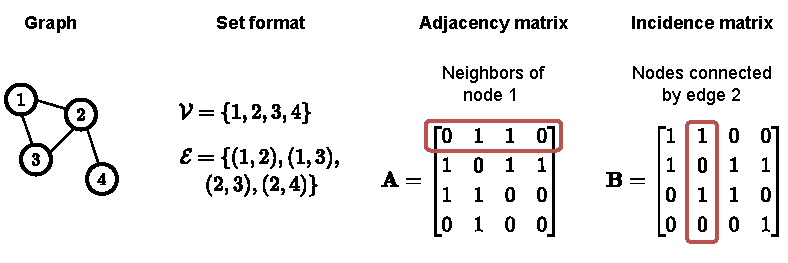
\includegraphics[width=1.0\textwidth]{images/graphs-2}
    \caption{Мы можем представить связность графа тремя способами: как множество $\mathcal{E}$ пар (второй столбец); как матрицу смежности $(n, n)$ (третий столбец); или как матрицу инцидентности $(n, \lvert \mathcal{E} \rvert)$ (четвертый столбец).}
    \label{fig:adjacency_matrix}
\end{figure}

Мы будем предполагать, что наши графы имеют петли, т.е. $A_{ii} = 1$. Если матрица смежности не имеет петель, мы можем добавить их, переназначив ее как:
%
$$\mathbf{A} \gets\mathbf{A} + \mathbf{I}$$

\subsection{Признаки графа}

Графы поставляются с множеством возможных признаков, описывающих их. Например, атомы и связи в молекуле могут быть описаны категориальными признаками, обозначающими их типы; дороги в транспортной сети могут иметь пропускную способность и транспортный поток; а два друга в социальных сетях могут быть описаны тем, сколько лет они знают друг друга.

В общем, эти признаки могут быть трех типов: \textbf{признаки узлов}, связанные с каждым узлом, \textbf{признаки ребер}, связанные с каждым ребром, и \textbf{признаки графа}, связанные со всем графом. Мы начнем с простейшего случая, когда у нас есть доступ только к неструктурированным признакам узлов, т.е. с каждым узлом $i$ связан вектор $\mathbf{x}_i \sim (c)$. Полный граф тогда можно описать двумя матрицами $\mathbf{X} \sim (n,c)$, которую мы называем \textbf{матрицей признаков}, и матрицей смежности $\mathbf{A} \sim (n,n)$.

В большинстве случаев порядок узлов не имеет значения, т.е. если мы рассмотрим матрицу перестановки $\mathbf{P} \sim \text{Binary}(n,n)$ (см. Раздел \ref{sec:positional_embeddings}), граф и его переставленная версия в основном идентичны, другими словами:

$$
(\mathbf{X}, \mathbf{A}) \;\; \text{ — это тот же граф, что и } \;\;(\mathbf{P}\mathbf{X},\mathbf{P}\mathbf{A}\mathbf{P}^\top)
$$

Обратите внимание, что матрица перестановки действует, меняя местами строки в $\mathbf{X}$, в то время как она меняет местами и строки, и столбцы в матрице смежности.

Некоторые признаки также можно извлечь непосредственно из топологии графа. Например, мы можем связать с каждым узлом скалярное значение $d_i$, называемое \textbf{степенью}, которое описывает, со сколькими узлами он соединен:

$$
d_i=\sum_j A_{ij}
$$

Распределение степеней по графу является важной характеристикой самого графа, как показано на Рисунке \ref{fig:random_graphs}. Мы можем собрать степени в одну диагональную матрицу, называемую матрицей \textbf{степеней}:

$$
\mathbf{D} =\begin{bmatrix} d_1 & \ldots & 0 \\ \vdots &\ddots & \vdots \\0 & \ldots & d_n \end{bmatrix}
$$

Мы можем использовать матрицу степеней для определения нескольких типов \textit{взвешенных} матриц смежности. Например, нормализованная по строкам матрица смежности определяется как:

$$
\mathbf{A}^\prime \leftarrow \mathbf{D}^{-1}\mathbf{A}_{ij} \;\; \rightarrow\;\; A^\prime_{ij} = \frac{1}{d_i}A_{ij}
$$



Это нормализовано в том смысле, что $\sum_i A^\prime_{ij} = \mathbf{1}$. Мы также можем определить нормализованную по столбцам матрицу смежности как $\mathbf{A}^\prime = \mathbf{A}\mathbf{D}^{-1}$. Обе эти матрицы можно интерпретировать как «случайные блуждания» по графу, в том смысле, что для данного узла $i$ соответствующая строка или столбец нормализованной матрицы смежности представляет собой распределение вероятностей случайного перемещения к любому из его соседей. Более общая симметрично нормализованная матрица смежности задается как:

$$
\mathbf{A}^\prime=\mathbf{D}^{-1/2}\mathbf{A}\mathbf{D}^{-1/2}
$$

Это определяется как $A^\prime_{ij} = \frac{A_{ij}}{\sqrt{d_i d_j}}$, придавая вес каждому соединению на основе степени обоих узлов, которые оно соединяет. И матрица смежности, и ее взвешенные варианты обладают свойством, что $A_{ij} = 0$, когда $(i,j) \notin \mathcal{E}$. В терминах обработки сигналов они называются \textbf{матрицами сдвига графа}.

\begin{supportbox}{Разреженность в матрицах}
Рассмотрим общую матрицу смежности для графа из 6 узлов (попробуйте нарисовать граф в качестве упражнения):
%
$$
\mathbf{A} = \begin{bmatrix} 0& 1& 1& 1& 1& 1\\1& 0& 0& 0& 1& 0\\1& 0& 0& 0& 1& 1\\1& 0& 0& 0& 0& 1\\1& 1& 1& 0& 0& 0\\1& 0& 1& 1& 0& 0\end{bmatrix}
$$

Смежность очень разрежена (много нулей). Это важное свойство, потому что разреженные матрицы имеют индивидуальные реализации и техники для их обработки, с лучшей вычислительной сложностью, чем у их плотных аналогов.\footnote{В качестве примера, в JAX: \url{https://jax.readthedocs.io/en/latest/jax.experimental.sparse.html}.}
\end{supportbox}

\begin{figure}[t]
    \centering
    \begin{subfigure}[b]{0.24\textwidth}
    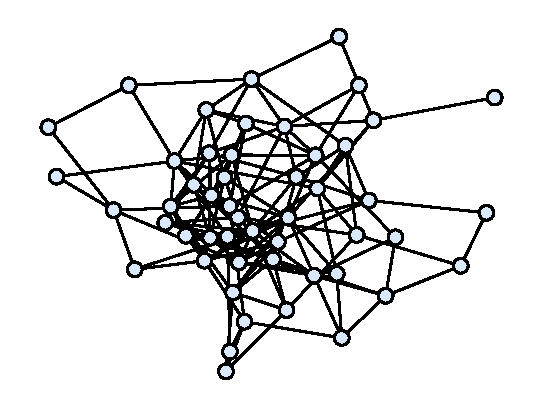
\includegraphics[width=\textwidth]{images/graph_1}
    \caption{Эрдёша-Реньи}
    \end{subfigure}
    \begin{subfigure}[b]{0.24\textwidth}
    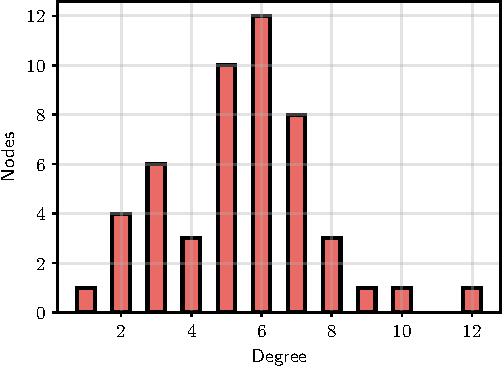
\includegraphics[width=\textwidth]{images/graph_1_degree}
    \caption{Степень}
    \end{subfigure}
    \begin{subfigure}[b]{0.24\textwidth}
    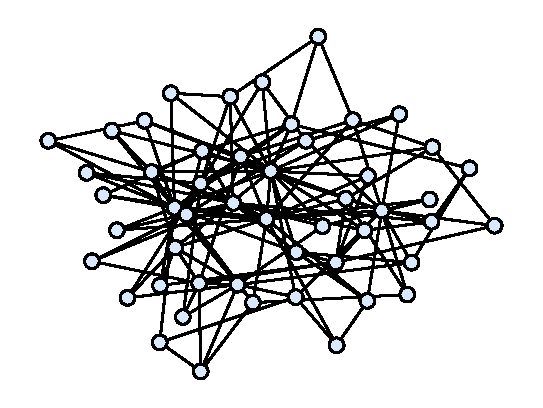
\includegraphics[width=\textwidth]{images/graph_2}
    \caption{Барабаши-Альберт}
    \end{subfigure}
    \begin{subfigure}[b]{0.24\textwidth}
    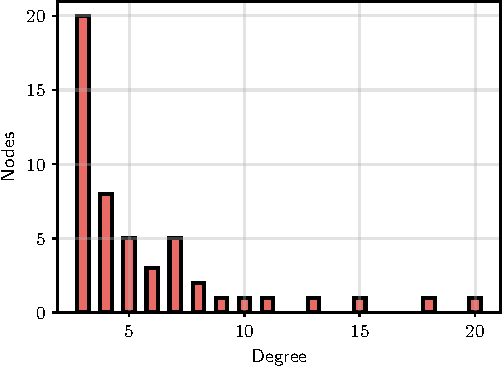
\includegraphics[width=\textwidth]{images/graph_2_degree}
    \caption{Степень}
    \end{subfigure}
    \caption{(a) Случайный граф, сгенерированный путем независимого выбора каждого ребра из распределения Бернулли (\textbf{модель Эрдёша-Реньи}). (b) Эти графы показывают гауссоподобное распределение степеней. (c) Случайный граф, сгенерированный путем последовательного добавления узлов, и для каждого из них выбора $3$ соединений с существующими узлами с вероятностью, пропорциональной их степени (\textbf{процесс предпочтительного присоединения} или \textbf{модель Барабаши-Альберта}). (d) Эти графы имеют несколько узлов с большим количеством соединений, действующих как хабы для графа.}
    \label{fig:random_graphs}
\end{figure}

\subsection{Операции диффузии по графам}

Основная операция на графе, которая нас интересует, — это так называемая \textbf{диффузия}, которая соответствует сглаживанию признаков узлов по отношению к топологии графа. Чтобы понять это, рассмотрим скалярный признак на каждом узле, который мы собираем в вектор $\mathbf{x} \sim (n)$, и следующую операцию над признаками:

$$
\mathbf{x}^\prime=\mathbf{A}\mathbf{x}
$$

где $\mathbf{A}$ может быть матрицей смежности, нормализованным вариантом или любой взвешенной матрицей смежности. Мы можем переписать эту операцию поузлово как:

$$
x^\prime_i = \sum_{j \in \mathcal{N}(i)} A_{ij}x_j
$$

где мы определили 1-скачковое соседство:

\vspace{1em}
$$
\mathcal{N}(i) = \left\{ j\mid \eqnmarkbox[drawred]{node}{(i,j)\in\mathcal{E}} \right\}
$$
\annotate[yshift=1em]{above,right}{node}{Все ребра с узлом $i$ в качестве вершины}

\vspace{-1em}
Если мы интерпретируем признак узла как физическую величину, проекцию на матрицу смежности можно рассматривать как процесс «диффузии», который заменяет величину в каждом узле взвешенным средним величины в его соседстве.

Другой фундаментальной матрицей в контексте анализа графов является \textbf{матрица Лапласа}:

$$
\mathbf{L}=\mathbf{D}-\mathbf{A}
$$

где матрица степеней вычисляется как $D_{ii} = \sum_j A_{ij}$ независимо от того, нормализована ли матрица смежности или нет. Один шаг диффузии с помощью Лапласиана можно записать как:

\begin{equation}
\mathbf{L}\mathbf{x}=\sum_{(i,j) \in \mathcal{E}} A_{ij}(x_i-x_j)
\label{eq:laplacian}
\end{equation}

\begin{figure}[t]
    \centering
    \begin{subfigure}[b]{0.24\textwidth}
    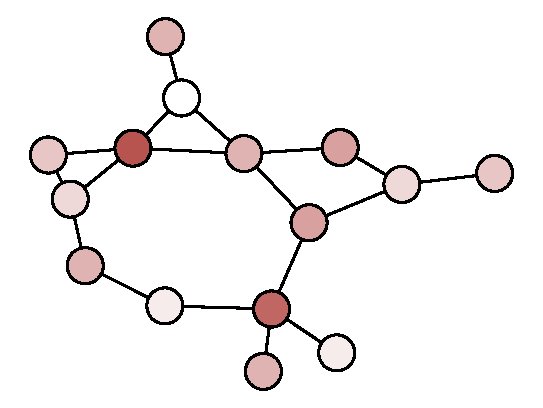
\includegraphics[width=\textwidth]{images/graph_diffusion_0}
    \caption{Исходный граф}
    \end{subfigure}
    \begin{subfigure}[b]{0.24\textwidth}
    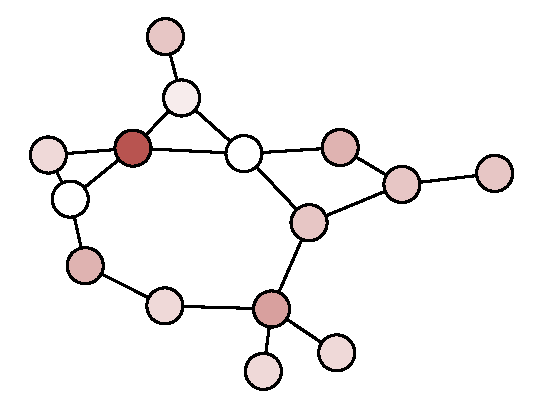
\includegraphics[width=\textwidth]{images/graph_diffusion_10}
    \caption{10 шагов}
    \end{subfigure}
    \begin{subfigure}[b]{0.24\textwidth}
    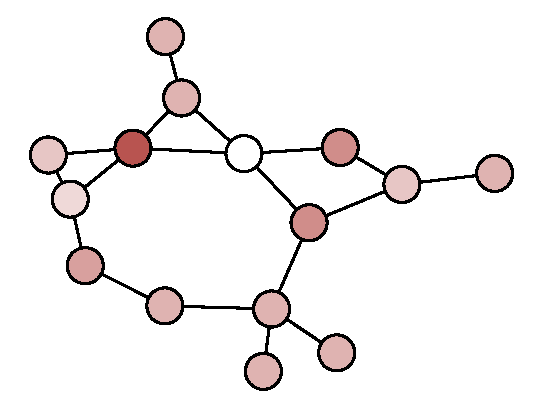
\includegraphics[width=\textwidth]{images/graph_diffusion_20}
    \caption{20 шагов}
    \end{subfigure}
    \begin{subfigure}[b]{0.24\textwidth}
    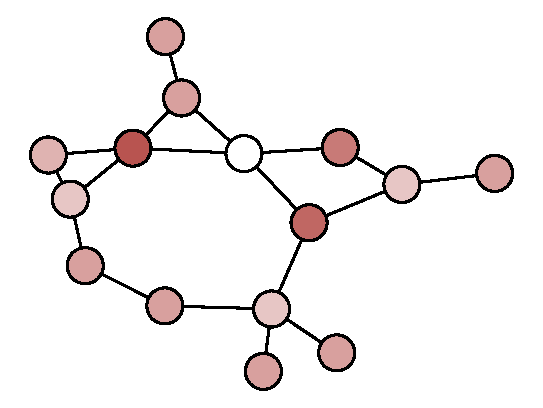
\includegraphics[width=\textwidth]{images/graph_diffusion_30}
    \caption{30 шагов}
    \end{subfigure}
    \caption{(a) Случайный граф с 15 узлами и скалярным признаком на каждом узле (обозначен разными цветами). (b)-(d) Результат после $10$, $20$ и $30$ шагов диффузии с матрицей Лапласа. Признаки сходятся к стабильному состоянию.}
    \label{fig:diffusion}
\end{figure}

Из этого мы видим, что Лапласиан тесно связан с идеей градиента на графе, и его анализ лежит в основе области \textbf{спектральной теории графов}. В качестве примера, в \eqref{eq:laplacian} $\mathbf{1}$ всегда является собственным вектором Лапласиана, связанным с нулевым собственным значением (в частности, наименьшим). Мы показываем пример диффузии с матрицей Лапласа на Рисунке \ref{fig:diffusion}.



\subsection{Регуляризация многообразия}

Из \eqref{eq:laplacian} мы также можем вывести квадратичную форму, построенную на Лапласиане:

\begin{equation}
\mathbf{x}^\top\mathbf{L}\mathbf{x}=\sum_{(i,j)\in \mathcal{E}}A_{ij}(x_i-x_j)^2
\label{eq:laplacian_regularizer}
\end{equation}

Неформально, это скалярное значение, которое измеряет, насколько «гладким» является сигнал на графе, т.е. как быстро он меняется для пар узлов, соединенных в графе. Чтобы увидеть простое применение этой концепции, рассмотрим табличный набор данных для классификации $\mathcal{S}_n = \left\{(\mathbf{x}_i, y_i)\right\}$. Предположим, мы строим граф на этом наборе данных, где каждый узел — это элемент набора данных, а матрица смежности строится на основе расстояния между признаками:

\begin{equation}
A_{ij}=\begin{cases} \exp(-\lVert \mathbf{x}_i - \mathbf{x}_j \rVert^2) & \text{ если } \lVert \mathbf{x}_i - \mathbf{x}_j \rVert^2 < \tau \\ 0 & \text{иначе} \end{cases}
\label{eq:dataset_graph}
\end{equation}

где $\tau$ — заданный пользователем гиперпараметр. Для классификационной модели $f(\mathbf{x})$ мы можем захотеть ограничить ее выход, чтобы он был схожим для схожих входов, где сходство определяется пропорционально \eqref{eq:dataset_graph}. Для этого мы можем определить признаки графа как выходы нашей модели:

$$
\mathbf{f} = \begin{bmatrix} f(\mathbf{x}_1) \\ \vdots \\ f(\mathbf{x}_n) \end{bmatrix} \sim (n)
$$

Квадратичная форма \eqref{eq:laplacian_regularizer} говорит нам, насколько сильно различаются схожие входы с точки зрения их предсказаний:

\begin{equation}
\mathbf{f}^\top\mathbf{L}\mathbf{f} = \sum_{i,j} A_{ij}(f(\mathbf{x}_i)-f(\mathbf{x}_j))^2
\label{eq:manifold_regularizer}
\end{equation}

Оптимальную модель можно найти с помощью регуляризованной задачи оптимизации, где регуляризатор задается как \eqref{eq:manifold_regularizer}:
%
$$
f^*(\mathbf{x})=\arg\min \left\{\sum_{i=1}^nL(y_i, f(\mathbf{x}))  + \lambda \;\;\mathbf{f}^\top \mathbf{L}\mathbf{f}\right\}
$$
%
где $L$ — общая функция потерь, а $\lambda$ — скалярный гиперпараметр:

Это называется \textbf{регуляризацией многообразия} \cite{belkin2006manifold} и может использоваться как общий инструмент регуляризации для принуждения модели быть гладкой на графе, где смежность либо задана, либо строится пользователем, как в \eqref{eq:dataset_graph}. Это особенно полезно в \textbf{полууправляемом} сценарии, где у нас есть небольшой размеченный набор данных и большой неразмеченный из того же распределения, поскольку регуляризатор в \eqref{eq:manifold_regularizer} не требует меток \cite{belkin2006manifold}. Однако предсказание модели зависит только от одного элемента $\mathbf{x}_i$, и граф отбрасывается после обучения. В следующем разделе мы представим более естественные способы встраивания связности в саму модель.

\section{Графовые свёрточные слои}
\subsection{Свойства графового слоя}

Чтобы спроектировать модели, чьи предсказания зависят от связности, мы можем дополнить стандартные слои $f(\mathbf{X})$ знанием матрицы смежности, т.е. мы рассматриваем слои вида:
%
$$
\mathbf{H} =f(\mathbf{X}, \mathbf{A})
$$
%
где, как и прежде, $\mathbf{X} \sim (n, c)$ (где $n$ — количество узлов, а $c$ — признаки в каждом узле) и $\mathbf{H} \sim (n, c^\prime)$, т.е. операция не изменяет связность графа, и она возвращает обновленное вложение $\mathbf{H}_i \sim (c^\prime)$ для каждого узла $i$ в графе. Для дальнейшего, $\mathbf{A}$ может быть матрицей смежности или любой матрицей с тем же паттерном разреженности (матрицей сдвига графа), включая взвешенную матрицу смежности, матрицу Лапласа и так далее.

Поскольку перестановка узлов в графе не должна влиять на конечные предсказания, слой не должен зависеть от конкретного порядка узлов, т.е. для любой матрицы перестановки $\mathbf{P}$ выход слоя должен быть \textbf{перестановочно эквивариантным}:
%
$$
f(\mathbf{P}\mathbf{X}, \mathbf{P}\mathbf{A}\mathbf{P}^\top)=\mathbf{P}\,\cdot\,f(\mathbf{X}, \mathbf{A})
$$
%
Мы можем определить понятие «локальности» для графового слоя, аналогично случаю с изображениями. Для этого мы сначала вводим понятие подграфа. Для подмножества узлов $\mathcal{T} \in \mathcal{V}$ из полного графа мы определяем \textbf{подграф}, индуцированный $\mathcal{T}$, как:
%
$$
\mathcal{G}_{\mathcal{T}}= (\mathbf{X}_{\mathcal{T}}, \mathbf{A}_{\mathcal{T}})
$$
%
где $\mathbf{X}_{\mathcal{T}}$ — это матрица $(\lvert\mathcal{T}\rvert,c)$, собирающая признаки узлов в $\mathcal{T}$, а $\mathbf{A} \sim (\lvert\mathcal{T}\rvert,\lvert\mathcal{T}\rvert)$ — соответствующий блок полной матрицы смежности.

\begin{definition}[Локальность графа]
Графовый слой $\mathbf{H} =f(\mathbf{X}, \mathbf{A})$ является \textbf{локальным}, если для каждого узла $\mathbf{H}_i = f(\mathbf{X}_{\mathcal{N}(i)}, \mathbf{A}_{\mathcal{N}(i)})$, где $\mathcal{N}(i)$ — это 1-скачковое соседство узла $i$.
\end{definition}

Это похоже на рассмотрение всех пикселей на расстоянии $1$ в случае с изображениями, за исключением того, что (а) узлы в $\mathcal{N}(i)$ в этом случае не имеют определенного порядка, и (б) размер $\mathcal{N}(i)$ может сильно варьироваться в зависимости от $i$. Следовательно, мы не можем определить свёртку, как мы это делали в случае с изображениями, поскольку ее определение требует этих двух свойств (подумайте о весовом тензоре в свёрточном слое).

Для дальнейшего, обратите внимание, что мы можем расширить наше определение локальности за пределы 1-скачковых соседей. Например, 2-скачковое соседство $\mathcal{N}^2(i)$ определяется как все узлы на расстоянии не более $2$:
%
$$
\mathcal{N}^2(i) = \bigcup_{j \in \mathcal{N}(i)} \mathcal{N}(j) 
$$
%
где $\cup$ — это оператор объединения множеств. Мы можем расширить определение локальности, чтобы учесть соседства более высокого порядка и спроектировать эквивалент фильтров $3 \times 3$, $5 \times 5$ и так далее.

\subsection{Графовый свёрточный слой} \addclock

Чтобы определить графовый слой, который имитирует свёрточный слой, нам нужно, чтобы он был перестановочно эквивариантным (вместо трансляционно эквивариантного) и локальным. Слой MHA естественно перестановочно эквивариантен, но он не является локальным и не зависит явно от матрицы смежности $\mathbf{A}$. Мы увидим возможные расширения для этого в следующем разделе. Пока давайте сосредоточимся на более простом полносвязном слое:
%
$$
f(\mathbf{X}, \_)= \phi(\mathbf{X}\mathbf{W}+\mathbf{b})
$$
%
где $\mathbf{W} \sim (c^\prime,c)$ и $\mathbf{b} \sim (c^\prime)$. Он также естественно перестановочно эквивариантен, но не зависит от связности графа, которая игнорируется. Чтобы построить соответствующий дифференцируемый слой, мы можем чередовать операцию слоя с шагом диффузии.

\begin{definition}[Графовая свёртка] \addbottle
%
Для графа, представленного матрицей признаков узлов $\mathbf{X} \sim (n,c)$ и общей матрицей сдвига графа $\mathbf{A} \sim (n,n)$ (смежность, Лапласиан, ...), \textbf{графовый свёрточный} (GC) слой задается как \cite{kipf2016semi}:
%
$$
f(\mathbf{X}, {\color{drawred}\mathbf{A}})= \phi({\color{drawred}\mathbf{A}}(\mathbf{X}\mathbf{W}+\mathbf{b}))
$$
%
где обучаемыми параметрами являются $\mathbf{W} \sim (c^\prime,c)$ и $\mathbf{b} \sim (c^\prime)$, где $c^\prime$ — гиперпараметр. $\phi$ — это стандартная функция активации, такая как ReLU.
\end{definition}

\begin{SCfigure}
    \centering
    \hspace{2em}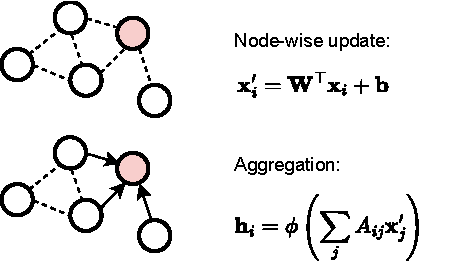
\includegraphics[width=0.5\textwidth]{images/graph_convolution_layer}
    \caption{Два этапа слоя GC: каждый узел обновляет свое вложение параллельно со всеми остальными узлами; выход задается взвешенным средним всех обновленных вложений в соседстве узла.}
    \label{fig:graph_convolution_layer}
\end{SCfigure}

Обратите внимание на сходство со стандартным свёрточным слоем: мы выполняем операцию «смешивания каналов» с помощью матрицы $\mathbf{W}$ и операцию «смешивания узлов» с помощью матрицы $\mathbf{A}$, разница в том, что первая в этом случае необучаема (из-за, опять же, переменных степеней между узлами и необходимости сделать слой перестановочно эквивариантным). См. Рисунок \ref{fig:graph_convolution_layer} для визуализации. Аналогию также можно более формально обосновать, используя понятия из обработки сигналов на графах, что выходит за рамки этой книги \cite{bronstein2017geometric}. Игнорируя смещение, мы можем переписать это для одного узла $i$ как:

$$
\mathbf{H}_i=\phi\left(\sum_{j \in \mathcal{N}(i)}A_{ij}\mathbf{X}_j\mathbf{W}\right)
$$

Следовательно, мы сначала выполняем одновременное обновление всех вложений узлов (заданное правым умножением на $\mathbf{W}$). Затем каждый узел вычисляет взвешенное среднее обновленных вложений узлов от себя и своих соседей. Поскольку количество соседей может варьироваться от узла к узлу, работа с нормализованными вариантами матрицы смежности может значительно помочь в обучении. Тривиально показать перестановочную эквивариантность для слоя:

$$
f({\color{drawred}\mathbf{P}}\mathbf{X},{\color{drawred}\mathbf{P}}\mathbf{A}{\color{drawred}\mathbf{P}^\top})=\phi\left({\color{drawred}\mathbf{P}}\mathbf{A}{\color{drawred}\mathbf{P}^\top}{\color{drawred}\mathbf{P}}\mathbf{X}\mathbf{W}\right) = {\color{drawred}\mathbf{P}}\,\cdot\,f(\mathbf{X},\mathbf{A})
$$

\subsection{Построение графовой свёрточной сети}

Один слой GC является локальным, но стек из нескольких слоев — нет. Например, рассмотрим двухслойную модель GC:

\begin{equation}
f(\mathbf{X},\mathbf{A})=\phi(\mathbf{A}\eqnmarkbox[drawred]{node}{\phi\left(\mathbf{A}\mathbf{X}\mathbf{W}_1\right)}\mathbf{W}_2)
\label{eq:two_layer_gcn}
\end{equation}
\annotate[yshift=-1em]{below,right}{node}{Первый слой GC}

\vspace{1em}
с двумя обучаемыми весовыми матрицами $\mathbf{W}_1$ и $\mathbf{W}_2$. Аналогично случаю с изображениями, мы можем определить понятие рецептивного поля.

\begin{definition}[Рецептивное поле графа]
Для общей графовой нейронной сети $\mathbf{H} = f(\mathbf{X}, \mathbf{A})$ \textbf{рецептивное поле} узла $i$ — это наименьшее множество узлов $\mathcal{V}(i) \in \mathcal{V}$, такое что $\mathbf{H}_i = f(\mathbf{X}_{\mathcal{V}(i)}, \mathbf{A}_{\mathcal{V}(i)})$.
\end{definition}

Для одного слоя GC рецептивное поле равно $\mathcal{V}(i) = \mathcal{N}(i)$. Для двухслойной сети, как в \eqref{eq:two_layer_gcn}, нам нужно рассматривать соседей соседей, и рецептивное поле становится $\mathcal{V}(i) = \mathcal{N}^2(i)$. В общем, для стека из $k$ слоев у нас будет рецептивное поле $\mathcal{V}(i) = \mathcal{N}^k(i)$. Наименьшее количество шагов, необходимое для перехода от любого узла к любому другому в графе, называется \textbf{диаметром} графа. Диаметр определяет наименьшее количество слоев, необходимое для достижения глобального рецептивного поля для всех узлов. 

\begin{supportbox}{Полиномиальные слои GC}

В качестве альтернативы мы можем увеличить рецептивное поле \textit{одного} слоя GC. Например, если мы удалим петли из матрицы смежности, мы можем сделать слой локальным по отношению к $\mathcal{N}^2(i)$ вместо $\mathcal{N}(i)$, также рассматривая квадрат матрицы смежности:

$$
\mathbf{H} = \phi\left(\mathbf{X}\mathbf{W}_0 + \mathbf{A}\mathbf{X}\mathbf{W}_1 + \mathbf{A}^2\mathbf{X}\mathbf{W}_2\right)
$$

где у нас есть три набора параметров $\mathbf{W}_0$, $\mathbf{W}_1$ и $\mathbf{W}_2$ для обработки петель, соседей и соседей соседей соответственно. Это называется \textbf{полиномиальным} слоем GC. Большие рецептивные поля можно получить с помощью более высоких степеней. Более сложные слои можно спроектировать, рассматривая отношения полиномов \cite{bianchi2021graph}.

\end{supportbox}

Мы можем комбинировать слои GC со стандартными слоями нормализации, остаточными соединениями, dropout или любой другой операцией, которая является перестановочно эквивариантной. В отличие от случая с изображениями, пулинг сложнее, потому что нет непосредственного способа подвыборки связности графа. Слои пулинга все еще можно определить, используя инструменты из теории графов или добавляя дополнительные обучаемые компоненты, но они менее распространены \cite{grattarola2022understanding}.

Обозначим через $\mathbf{H} = f(\mathbf{X}, \mathbf{A})$ общую комбинацию слоев, предоставляющую обновленное вложение для каждого узла (без изменения связности). По аналогии с СНС, мы называем ее \textbf{основой} сети. Мы можем завершить проектирование общей \textbf{графовой свёрточной сети} (GCN), добавив небольшую голову поверх этих представлений:
%
$$
y=(g\circ f)(\mathbf{X},\mathbf{A})
$$
%
Дизайн головы зависит от задачи, которую мы пытаемся решить. Наиболее распространенные задачи делятся на одну из трех основных категорий: задачи на уровне узлов (например, классификация узлов), задачи на уровне ребер (например, классификация ребер) или задачи на уровне графа (например, классификация графа). Мы кратко рассмотрим пример для каждой из них по очереди, см. Рисунок \ref{fig:graph_heads}.

\begin{figure}[t]
    \centering
    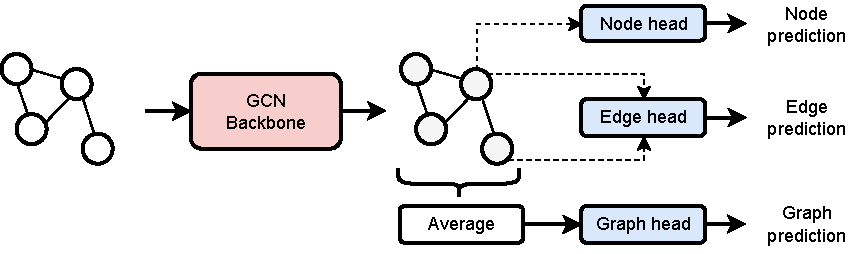
\includegraphics[width=0.9\textwidth]{images/graph_heads}
    \caption{Различные типы графовых голов: (a) задачи на узлах требуют обработки признаков одного узла; (b) задачи на ребрах требуют голов, которые зависят от двух узлов одновременно; (c) задачи на графах можно решить, объединив все представления узлов в вектор фиксированной размерности.}
    \label{fig:graph_heads}
\end{figure}

\textbf{Классификация узлов}

Во-первых, предположим, что входной граф описывает некоторую социальную сеть, где каждый пользователь связан с узлом. Для заданного подмножества пользователей, $\mathcal{T} \subseteq \mathcal{V}$, мы знаем метку $y_i, i \in \mathcal{T}$ (например, является ли пользователь реальным пользователем, ботом или другим типом автоматизированного профиля). Нас интересует предсказание метки для всех остальных узлов. В этом случае мы можем получить поузловое предсказание, обработав каждое обновленное вложение узла, например:

$$
\hat{y}_i=g(\mathbf{H}_i) =\text{softmax}(\text{MLP}(\mathbf{H}_i))
$$

Выполнение этой операции над всей матрицей $\mathbf{H}$ дает нам предсказание для всех узлов, но мы знаем истинные метки только для небольшого подмножества. Мы можем обучать GCN, отбрасывая узлы за пределами обучающего набора:

$$
\arg\min \frac{1}{\lvert \mathcal{T} \rvert}\sum_{i \in \mathcal{T}} \text{CE}(\hat{y}_i,y_i)
$$

где $\text{CE}$ — это кросс-энтропийная потеря. Важно, что даже если мы отбрасываем выходные предсказания для узлов за пределами нашего обучающего набора, их входные признаки все еще участвуют в процессе обучения из-за шагов диффузии внутри GCN. Остальные узлы затем можно классифицировать, запустив GCN в последний раз после обучения. Этот сценарий, где размечена только часть обучающих данных, называется \textbf{полууправляемой} задачей.

\textbf{Классификация ребер}

В качестве второго примера, предположим, у нас есть метка для подмножества \textit{ребер}, т.е. $\mathcal{T}_E \subseteq \mathcal{E}$. Например, наш граф может быть транспортной сетью, для которой мы знаем транспортный поток только на подмножестве дорог. В этом случае мы можем получить пореберное предсказание, добавив голову, которая зависит от признаков двух соединенных узлов, например, объединив их:

$$
\hat{y}_{ij} = g(\mathbf{H}_i, \mathbf{H}_j)= \text{MLP}\left(\left[ \mathbf{H}_i \;\Vert \; \mathbf{H}_j\right]\right)
$$

Для бинарной классификации (например, предсказания близости двух пользователей со скалярным значением от $0$ до $1$) мы можем упростить это, рассмотрев скалярное произведение двух признаков:

$$
\hat{y}_{ij} = \sigma( \mathbf{H}_i^\top \mathbf{H}_j)
$$

Как и прежде, мы можем обучать сеть, минимизируя потери по известным ребрам.

\textbf{Классификация графов}

Наконец, предположим, нас интересует классификация (или регрессия) всего графа. Например, граф может быть молекулой, для которой мы хотим предсказать некоторое химическое свойство, такое как реакционная способность по отношению к данному соединению. Мы можем достичь этого, объединив представления узлов (например, с помощью суммы) и обработав результирующее вложение фиксированной размерности:

$$
y=\text{MLP}\left(\frac{1}{n}\sum_{i=1}^n \mathbf{H}_i\right)
$$

Последний слой пулинга делает сеть \textit{инвариантной} к перестановке узлов. В этом случае наш набор данных будет состоять из нескольких графов (например, нескольких молекул), что делает его похожим на стандартную задачу классификации изображений. Для задач на узлах и ребрах, напротив, некоторые наборы данных могут состоять из одного графа (например, большой социальной сети), в то время как другие наборы данных могут иметь более одного графа (например, несколько несвязанных дорожных сетей из разных городов). Это открывает вопрос о том, как эффективно строить мини-пакеты графов.

\subsection{О реализации графовых нейронных сетей} \addteacup

Как мы уже упоминали, особенность работы с графами заключается в том, что несколько матриц, участвующих в наших вычислениях, могут быть очень разреженными. Например, рассмотрим следующую матрицу смежности:

$$
\mathbf{A} = \begin{bmatrix} 0 & 0 & 1 \\ 0 & 0 & 0 \\ 1 & 0 & 0 \end{bmatrix}
$$

Это соответствует графу из трех узлов с одним двунаправленным ребром между узлами $1$ и $3$. Мы можем хранить это более эффективно, сохраняя только индексы ненулевых значений, например, в коде:

{\begin{center}\footnotesize
\noindent\mintinline{python}{A = [[0,2], [2,0]]}
\end{center}
}

Это называется форматом \textbf{списка координат}. Для очень разреженных матриц специализированные форматы, подобные этому, могут уменьшить объем хранения, а также значительно улучшить время выполнения операций над разреженными матрицами или над комбинациями разреженных и плотных матриц. В качестве примера, pytorch-sparse\footnote{\url{https://github.com/rusty1s/pytorch_sparse}} поддерживает высокоэффективные реализации транспонирования и нескольких типов умножения матриц в PyTorch. Это также отражается на реализации слоев. Прямой проход слоев в PyTorch Geometric\footnote{\url{https://pytorch-geometric.readthedocs.io/en/latest/get_started/introduction.html\#learning-methods-on-graphs}} (одна из самых распространенных библиотек для работы с графовыми нейронными сетями в PyTorch) параметризуется путем предоставления в качестве входов признаков графа и связности в виде списка координат ребер.

\begin{SCfigure}
    \centering
    \hspace{2em}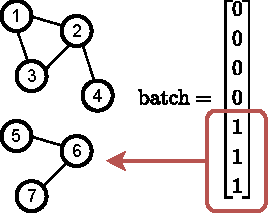
\includegraphics[width=0.4\textwidth]{images/graphs-Page-4}
    \caption{Два графа в мини-пакете можно рассматривать как один граф с двумя несвязанными компонентами. Чтобы их различить, нам нужно ввести дополнительный вектор, содержащий отображение между узлами и идентификаторами графов.}
    \label{fig:graph_batch}
\end{SCfigure}

Работа с разреженными матрицами имеет еще одно интересное следствие с точки зрения мини-пакетов. Предположим, у нас есть $b$ графов $(\mathbf{X}_i, \mathbf{A}_i)_{i=1}^b$. Для каждого графа у нас одинаковое количество признаков узлов $c$, но разное количество узлов $n_i$, так что $\mathbf{X}_i \sim (n_i, c)$ и $\mathbf{A}_i \sim \text{Binary}(n_i, n_i)$. Чтобы построить мини-пакет, мы можем создать два тензора 3-го ранга:
%
\begin{gather}
X \sim (b,n,c) \\A\sim \text{Binary}(b,n,n)
\end{gather}
%
где $n = \max(n_1, \ldots, n_b)$, и обе матрицы дополняются нулями, чтобы заполнить два тензора. Однако более элегантную альтернативу можно получить, заметив, что в слое GC два узла, которые не соединены никаким путем (последовательностью ребер), никогда не будут общаться. Следовательно, мы можем построить \textit{один} граф, описывающий весь мини-пакет, просто объединив все узлы:
%
\begin{gather}
\mathbf{X} = \begin{bmatrix}\mathbf{X}_1 \\ \vdots \\ \mathbf{X}_b \end{bmatrix} \\ \mathbf{A} = \begin{bmatrix} \mathbf{A}_1 & \ldots & \mathbf{0} \\ \vdots& \ddots & \vdots \\ \mathbf{0} & \ldots & \mathbf{A}_b \end{bmatrix}
\end{gather}
%
где $\mathbf{X} \sim (\sum_i n_i, c)$ и $\mathbf{A} \sim \text{Binary}(\sum_i n_i, \sum_i n_i)$. Матрица смежности мини-пакета имеет блочно-диагональную структуру, где все элементы вне диагональных блоков равны нулю (узлы из разных графов не соединены). Хотя это кажется расточительным, на самом деле это увеличивает коэффициент разреженности графа, что позволяет лучше использовать операции с разреженными матрицами. Следовательно, для наборов данных графов во многих случаях нет реальной разницы между работой с одним графом или мини-пакетом графов.

Чтобы отслеживать, какой узел принадлежит какому входному графу, мы можем дополнить представление дополнительным вектором $\mathbf{b} \sim (\sum_i n_i)$, таким что $b_i$ — это индекс в $[1, \ldots, b]$, идентифицирующий один из $b$ входных графов - см. Рисунок \ref{fig:graph_batch}. Для классификации графов мы можем использовать $\mathbf{b}$ для выполнения пулинга отдельно по группам узлов, соответствующим разным графам. Предположим, $\mathbf{H} \sim (n,c^\prime)$ — это выход основы GCN, тогда:
%
\begin{equation}
\text{scatter\_sum}\left(\mathbf{H}, \mathbf{b}\right) = \mathbf{Y} \sim (b, c^\prime)
\label{eq:scatter_sum}
\end{equation}
%
называется операцией \textbf{рассеянной суммы} и такова, что $\mathbf{Y}_i$ — это сумма всех строк $\mathbf{H}$, таких что $b_j = i$, как показано на Рисунке \ref{fig:scatter_sum}. Аналогичные операции можно определить для других типов операций пулинга, таких как средние и максимумы.

\begin{figure}[t]
    \centering
    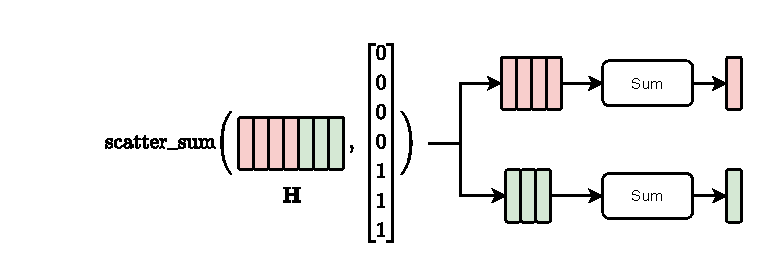
\includegraphics[width=0.9\textwidth]{images/graphs-Pagina-5}\hspace*{5em}
    \caption{Пример рассеянной суммы на графе с Рисунка \ref{fig:graph_batch}. В этом примере узлы (1,2,3,4) принадлежат графу 1, а узлы (5,6,7) — графу 2. После пулинга мы получаем объединенное представление для каждого из двух графов.}
    \label{fig:scatter_sum}
\end{figure}

В качестве отдельной проблемы, иногда у нас может быть один граф, который не помещается в память: в этом случае мини-пакеты должны формироваться путем \textit{выборки} подграфов из исходного графа \cite{hamilton2017inductive}. Это относительно сложная задача, которая выходит за рамки этой главы.

\section{За пределами графовых свёрточных слоев}

Имея слой GC в качестве шаблона, мы теперь рассмотрим несколько расширений, либо с точки зрения адаптивности, либо с точки зрения признаков графа, которые можно обрабатывать. В заключение мы обсудим \textbf{графовые трансформеры}, другое семейство слоев, в котором граф вкладывается в структурное вложение, которое суммируется с признаками узлов.

\subsection{Графовые слои внимания}

Одна из проблем со слоями GC заключается в том, что веса, которые используются для суммирования вкладов от соседей, фиксированы и задаются матрицей смежности (или соответствующим нормализованным вариантом). В большинстве случаев это эквивалентно предположению, что, за исключением относительного количества соединений, все соседи одинаково важны. Граф, в котором узлы в основном соединены с похожими узлами, называется \textbf{гомофильным}: эмпирически, гомофилия является хорошим предиктором производительности графовых свёрточных слоев \cite{li2022graph}. Не все графы гомофильны: например, в сети знакомств большинство людей будут соединены с людьми противоположного пола. Следовательно, в этих сценариях нам нужны техники, которые могут правильно адаптировать веса, заданные от одного узла к другому, адаптивно.

Для достаточно малых графов мы можем позволить ненулевым элементам весовой матрицы $\mathbf{A}$ адаптироваться от их начального значения с помощью градиентного спуска. Однако количество обучаемых параметров в этом случае увеличивается квадратично с числом узлов, и это решение не применимо к сценарию с более чем одним графом. Если мы предположим, что ребро зависит только от признаков двух узлов, которые оно соединяет, мы можем обобщить слой GC с помощью оператора, подобного вниманию:
%
$$
\mathbf{h}_i=\phi\left(\sum_{j \in \mathcal{N}(i)}{\color{drawred}\text{softmax}(\alpha(\mathbf{x}_i, \mathbf{x}_j))}\mathbf{W}^\top\mathbf{x}_j\right)
$$
%
где $\alpha$ — это некоторый общий блок МЛП, имеющий два входа и скалярный выход, а softmax применяется для каждого узла к набору выходов $\alpha$ по отношению к $\mathcal{N}(i)$, чтобы нормализовать веса независимо от размера соседства. Из-за сходства со слоем внимания они называются слоями \textbf{графового внимания} (GAT) \cite{velivckovic2017graph}. С точки зрения всего графа, это очень похоже на слой MHA, где операция внимания ограничена только узлами, имеющими ребро, которое их соединяет.

Выбор $\alpha$ относительно свободен. Вместо скалярного произведения, оригинальная формулировка GAT рассматривала МЛП, применяемый к конкатенации признаков:
%
$$
\alpha(\mathbf{x}_i, \mathbf{x}_j)=\text{LeakyReLU}(\mathbf{a}^\top \left[ \mathbf{V}\mathbf{x}_i \;\lVert\; \mathbf{V}\mathbf{x}_j \right])
$$
%
где $\mathbf{V}$ и $\mathbf{a}$ обучаемы. Позже было обнаружено, что это ограничивает, в том смысле, что порядок между элементами не зависит от центрального узла \cite{brody2021attentive}. Менее ограничительный вариант, называемый \textbf{GATv2} \cite{brody2021attentive}, получается как:
%
$$
\alpha(\mathbf{x}_i, \mathbf{x}_j)= \mathbf{a}^\top\text{LeakyReLU}( \mathbf{V}\left[ \mathbf{x}_i \;\lVert\; \mathbf{x}_j \right])
$$
%
И GAT, и GATv2 сегодня являются очень популярными базовыми линиями.

\subsection{Нейронные сети с передачей сообщений} \addteacup

Предположим, у нас есть дополнительные \textbf{признаки ребер} $\mathbf{e}_{ij}$, например, в наборе данных молекул мы можем знать one-hot закодированное представление типа каждой молекулярной связи. Мы можем обобщить слой GAT, чтобы включить эти признаки, правильно изменив функцию внимания:
%
$$
\alpha(\mathbf{x}_i, \mathbf{x}_j)= \mathbf{a}^\top\text{LeakyReLU}( \mathbf{V}\left[ \mathbf{x}_i \;\lVert\; \mathbf{x}_j \;\Vert\; {\color{drawred}\mathbf{e}_{ij}} \right])
$$
%
Мы можем еще больше обобщить все слои, рассмотренные до сих пор (GC, GAT, GATv2, GAT с признаками ребер), абстрагируясь от их основных компонентов. Рассмотрим очень общую формулировку слоя:
%
\begin{equation}
\mathbf{h}_i =\psi\left(\mathbf{x}_i, \text{Aggr}\left(\left\{M(\mathbf{x}_i, \mathbf{x}_j, \mathbf{e}_{ij})\right\}_{\mathcal{N}(i)}\right) \right)
\label{eq:message_passing_layer}
\end{equation}
%
где:
%
\begin{enumerate}
\item $M$ строит вектор признаков (который мы называем \textbf{сообщением}) относительно ребра между узлами $i$ и $j$. В отличие от слоев GC и GAT, мы не ограничиваем сообщение скалярным значением.
\item $\text{Aggr}$ — это общая перестановочно инвариантная функция (например, сумма) для агрегации сообщений от всех узлов, соединенных с узлом $i$.
\item $\psi$ — это заключительный блок, который объединяет агрегированное сообщение с признаками узла $\mathbf{x}_i$. Таким образом, два узла с одинаковым соседством все еще можно различить.
\end{enumerate}

В качестве примера, в слое GC сообщение строится как $M(\_, \mathbf{x}_j, \_)=A_{ij}\mathbf{W}^\top\mathbf{x}_j$, агрегация — это простая сумма, а $\psi(\_, \mathbf{x})=\phi(\mathbf{x})$. Общий слой \eqref{eq:message_passing_layer} был введен в \cite{gilmer2017neural} под названием слоя \textbf{передачи сообщений} и стал очень популярным способом классификации (и обобщения) слоев, работающих с графами \cite{velivckovic2022message}.

Давайте рассмотрим несколько примеров использования этой схемы передачи сообщений. Во-первых, мы можем захотеть уделить больше внимания центральному узлу на этапе передачи сообщений. Мы можем сделать это, изменив функцию $\psi$:
%
$$
\psi(\mathbf{x}, \mathbf{m})=\phi(\mathbf{V}\mathbf{x}+\mathbf{m})
$$
%
где $\mathbf{V}$ — это в общем обучаемая матрица (это было введено в \cite{morris2019weisfeiler} и популяризировано в PyTorch Geometric как слой GraphConv\footnote{\url{https://pytorch-geometric.readthedocs.io/en/latest/generated/torch_geometric.nn.conv.GraphConv.html}}). Во-вторых, предположим, что узлы имеют более сложные признаки, такие как временной ряд для каждого узла (например, распределенный набор датчиков). Обратите внимание, что в схеме передачи сообщений поузловые операции отделены от способа агрегации и обработки сообщений. Обозначая через $x_i$ временной ряд в узле $i$, мы можем обобщить слой GC, просто изменив функцию сообщения на слой, работающий с временными рядами, например, слой Conv1d:
%
$$
h_i=\sum_{j \in \mathcal{N}(i)} A_{ij} \text{Conv1d}(x_i)
$$
%
Это пример \textbf{пространственно-временного} слоя GC \cite{yu2017spatio}. Кроме того, до сих пор мы предполагали, что обновляться должны только признаки узлов. Однако легко также обновлять признаки ребер с помощью дополнительного слоя обновления ребер:
%
$$
\mathbf{e}_{ij} \leftarrow\text{MLP}(\mathbf{e}_{ij},\mathbf{h}_i, \mathbf{h}_j)
$$
%
Это также можно рассматривать как итерацию передачи сообщений, в которой ребро агрегирует сообщения от своих соседей (двух соединенных узлов). Эта линия рассуждений позволяет еще больше обобщить эти слои, чтобы рассматривать более расширенные соседства и признаки графа \cite{battaglia2018relational}.

Это очень краткий обзор, который дает представление о многих возможных вариантах передачи сообщений. Есть много тем, которые мы не можем подробно рассмотреть из-за нехватки места: среди них мы выделяем построение слоев MP для графов более высокого порядка (в которых ребра соединяют более чем пару узлов) \cite{chien2021you} и слоев MP для данных облаков точек, в которых нас интересует удовлетворение дополнительных симметрий (вращательных и трансляционных симметрий) \cite{satorras2021n,eijkelboom2023n}.

\subsection{Графовые трансформеры}

Мы рассмотрели две техники использования структуры графа: одна — добавить член регуляризации, который заставляет выходы сети быть гладкими по отношению к графу; вторая — ограничить операции графа следовать связности графа. В частности, в слое GAT мы использовали стандартную операцию внимания, правильно маскируя попарные сравнения. Однако мы также видели в предыдущей главе, что трансформеры стали популярны, потому что они предоставляют архитектуру, которая полностью агностична к типу данных. Можем ли мы спроектировать эквивалент \textbf{графового трансформера} \cite{muller2023attending}?

Напомним, что два основных шага для построения трансформера — это токенизация входных данных и определение позиционного вложения. Токенизация для графа проста: например, мы можем рассматривать каждый узел как токен, или (если заданы признаки ребер) каждый узел и каждое ребро как отдельные токены после их вложения в общее пространство. Давайте пока проигнорируем признаки ребер. Рассмотрим общую архитектуру, принимающую на вход признаки узлов:
%
$$
\mathbf{H} = \text{Transformer}(\mathbf{X})
$$
%
Она перестановочно эквивариантна, но полностью агностична к связности. Мы можем частично решить эту проблему, дополнив признаки узлов некоторыми графовыми признаками, такими как степень узла или кратчайшее расстояние до некоторых предварительно выбранных узлов (якорей) \cite{rampavsek2022recipe,muller2023attending}. Однако в более общем смысле мы можем рассмотреть вложение связности графа в то, что мы называем \textbf{структурным вложением}:
%
$$
\mathbf{H} = \text{Transformer}(\mathbf{X} + \text{Embedding}(\mathbf{A}))
$$

\begin{SCfigure}
    \centering
    \hspace{1em}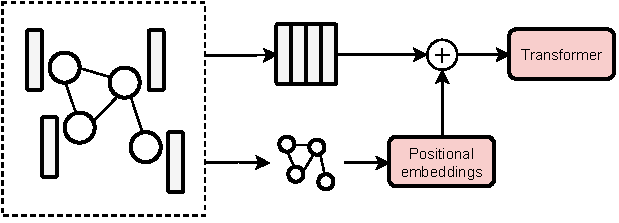
\includegraphics[width=0.6\textwidth]{images/graph_transformer}
    \caption{Общая идея графового трансформера: связность вкладывается в набор позиционных вложений, которые добавляются к собранным признакам. Результат затем обрабатывается стандартной сетью-трансформером.}
    \label{fig:graph_transformer}
\end{SCfigure}

Каждая строка $\text{Embedding}(\mathbf{A})$ предоставляет векторное вложение связности графа относительно одного узла, игнорируя все признаки (см. Рисунок \ref{fig:graph_transformer}). К счастью, вложение структуры графа в векторное пространство — это обширная область. В качестве примера мы опишем здесь распространенную процедуру вложения, основанную на случайных блужданиях \cite{dwivedi2021graph}. Напомним, что следующая матрица:
%
$$
\mathbf{R} =\mathbf{A}\mathbf{D}^{-1}
$$
%
может быть интерпретирована как «случайное блуждание», в котором $R_{ij}$ — это вероятность перехода от узла $i$ к узлу $j$. Мы можем итерировать случайное блуждание несколько раз, для фиксированного $k$, заданного априори пользователем:
%
$$
\mathbf{R}, \mathbf{R}^2, \ldots,\mathbf{R}^k
$$
%
Вложения случайных блужданий строятся путем сбора всех вероятностей блуждания узла, возвращающегося к себе, и проецирования их в вложение фиксированной размерности:
%
$$
\text{Embedding}(\mathbf{A})=\begin{bmatrix} \text{diag}(\mathbf{R}) \\ \text{diag}(\mathbf{R}^2) \\ \vdots \\ \text{diag}(\mathbf{R}^k)\end{bmatrix}\mathbf{W}
$$
%
При определенных условиях на структуру графа можно показать, что это обеспечивает уникальное представление для каждого узла \cite{dwivedi2021graph}. Альтернативные типы вложений можно получить, рассматривая собственные разложения матрицы Лапласа \cite{lim2022sign}. Для более полного изложения графовых трансформеров мы отсылаем к \cite{muller2023attending}. Построение графовых трансформеров открывает возможность для моделей-оснований типа GPT для графовой области, а также для добавления графовых данных в качестве дополнительной модальности к существующим языковым моделям \cite{maoposition}.

\section*{От теории к практике}

\begin{wrapfigure}{r}{3.0cm}
\vspace{-5em}
\includegraphics[width=3.0cm]{images/shutterstock_2075221579.jpg}
\vspace{-2em}
\end{wrapfigure}

Эффективная обработка графовых данных требует расширений базовых фреймворков из-за проблем, описанных в этой главе (например, разреженность). Распространенные библиотеки включают PyTorch Geometric для PyTorch и Jraph для JAX. Обе имеют обширные наборы руководств, например, для классификации узлов в небольших сетях цитирования.\footnote{Рекомендуемый пример в PyTorch Geometric: \url{https://pytorch-geometric.readthedocs.io/en/latest/get_started/introduction.html}.}

\begin{SCfigure}
    \centering
    \hspace{1em}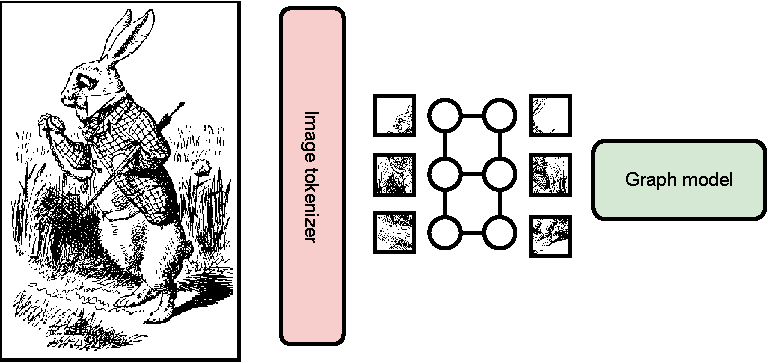
\includegraphics[width=0.6\textwidth]{images/ImageGNN}
    \caption{GNN для компьютерного зрения: изображение токенизируется на патчи, строится матрица смежности по патчам, и они оба передаются через графовую модель.}
    \label{fig:image_gnn}
\end{SCfigure}

Если вы реализовали Vision Transformer в Главе \ref{chap:transformers_in_practice}, я предлагаю забавное упражнение, которое имеет (в основном) дидактическую ценность, как показано на Рисунке \ref{fig:image_gnn}. Предположим, мы токенизируем изображение на патчи, но вместо добавления позиционных вложений мы строим матрицу смежности $\mathbf{A} \sim (p, p)$ (где $p$ — количество патчей) как:
%
\begin{equation}
A_{ij} = \begin{cases} 1 & \text{ если два патча имеют общую границу на изображении} \\ 0 & \text{ иначе} \end{cases}
\label{eq:image_adjacency_matrix}
\end{equation}

Теперь у нас есть набор данных для классификации графов, где признаки узлов задаются вложением патчей, а матрица смежности — \eqref{eq:image_adjacency_matrix}. Таким образом, мы можем выполнять классификацию изображений, адаптируя GNN из ранее упомянутых руководств.